%%%%%%%%%%%%%%%%%%%%%%%%
%% Sample use of the infthesis class to prepare a thesis. This can be used as
%% a template to produce your own thesis.
%%
%% The title, abstract and so on are taken from Martin Reddy's csthesis class
%% documentation.
%%
%% MEF, October 2002
%%%%%%%%%%%%%%%%%%%%%%%%

%%%%
%% Load the class. Put any options that you want here (see the documentation
%% for the list of options). The following are samples for each type of
%% thesis:
%%
%% Note: you can also specify any of the following options:
%%  logo: put a University of Edinburgh logo onto the title page
%%  frontabs: put the abstract onto the title page
%%  deptreport: produce a title page that fits into a Computer Science
%%      departmental cover [not sure if this actually works]
%%  singlespacing, fullspacing, doublespacing: choose line spacing
%%  oneside, twoside: specify a one-sided or two-sided thesis
%%  10pt, 11pt, 12pt: choose a font size
%%  centrechapter, leftchapter, rightchapter: alignment of chapter headings
%%  sansheadings, normalheadings: headings and captions in sans-serif
%%      (default) or in the same font as the rest of the thesis
%%  [no]listsintoc: put list of figures/tables in table of contents (default:
%%      not)
%%  romanprepages, plainprepages: number the preliminary pages with Roman
%%      numerals (default) or consecutively with the rest of the thesis
%%  parskip: don't indent paragraphs, put a blank line between instead
%%  abbrevs: define a list of useful abbreviations (see documentation)
%%  draft: produce a single-spaced, double-sided thesis with narrow margins
%%
%% For a PhD thesis -- you must also specify a research institute:
\documentclass[msc, ai, logo, deptreport, oneside, fullpacing]{infthesis}

%% For an MPhil thesis -- also needs an institute
% \documentclass[mphil,ianc]{infthesis}

%% MSc by Research, which also needs an institute
% \documentclass[mscres,irr]{infthesis}

%% Taught MSc -- specify a particular degree instead. If none is specified,
%% "MSc in Informatics" is used.
% \documentclass[msc,cogsci]{infthesis}
% \documentclass[msc]{infthesis}  % for the MSc in Informatics

%% Master of Informatics (5 year degree)
% \documentclass[minf]{infthesis}

%% Undergraduate project -- specify the degree course and project type
%% separately
% \documentclass[bsc]{infthesis}
% \course{Artificial Intelligence and Psychology}
% \project{Fourth Year Project Report}

%% Put any \usepackage commands you want to use right here; the following is
%% an example:
\usepackage{natbib}
\usepackage{graphicx}
\usepackage{amsmath}
\usepackage{url}
% Merge cells in table
\usepackage{multirow}

% For quotes
\usepackage{csquotes}

% For size of cells in tables
\usepackage{array}
\newcolumntype{S}[1]{>{\raggedright\let\newline\\\arraybackslash\hspace{0pt}}m{#1}}
\newcolumntype{R}[1]{>{\raggedright\let\newline\\\arraybackslash\hspace{1pt}}m{#1}}
% \newcolumntype{R}[1]{>{\centering\arraybackslash\hspace{1pt}}p{#1}}


%% Information about the title, etc.
\title{Gamifying Spaced Repetition Software}
\author{Sebastian Velasquez}

%% If the year of submission is not the current year, uncomment this line and
%% specify it here:
% \submityear{1785}

%% Optionally, specify the graduation month and year:
% \graduationdate{February 1786}

%% Specify the abstract here.
\abstract{%
Anki is a software system that implements spaced repetition. Despite its popularity, its interface for Android devices, known as AnkiDroid, lacks the inclusion of extrinsic motivational elements. Gamification involves the inclusion of game elements and schemes in non-game contexts; its objective is to improve the user experience by providing extra motivational elements in existing tools. The present work provides a gamification strategy aimed at increasing user engagement in AnkiDroid. The key difference from other gamification options is the inclusion of a casual game. The project consists of the design and implementation of the gamification solution, the definition and execution of a study to collect data, and the evaluation of the solution. The results showed that there was no statistically significant difference between a traditional gamification scheme and the proposed one. Those results served as the basis to discuss potential issues in the design and suggest additional work.
}

%% Now we start with the actual document.
\begin{document}

%% First, the preliminary pages
\begin{preliminary}

%% This creates the title page
\maketitle

%% Acknowledgements
\begin{acknowledgements}
Thanks to Dr. Hugh Leather and Dr. Volver Seeker for their supervision and guidance. Thanks to Dr. Kami Vaniea for her suggestions on user interface modifications. Thanks to Dr. Rafael Correa for his support to higher education in Ecuador. Special thanks to my family for their support during my studies.
\end{acknowledgements}

%% Next we need to have the declaration.
\standarddeclaration

%% Finally, a dedication (this is optional -- uncomment the following line if
%% you want one).
\dedication{To Milena and Gabriela.}

%% Create the table of contents
\tableofcontents

%% If you want a list of figures or tables, uncomment the appropriate line(s)
\listoffigures
\listoftables

\end{preliminary}

%%%%%%%%
%% Include your chapter files here. See the sample chapter file for the basic
%% format.
% Chapter 1

\chapter{Introduction} % Main chapter title

\label{intro} % For referencing the chapter elsewhere, use \ref{Chapter1} 

\lhead{Chapter 1. \emph{Introduction}} % This is for the header on each page - perhaps a shortened title

%----------------------------------------------------------------------------------------
\section{Gamification}
Gamification can be defined as the process of adding game elements and mechanics in non-game contexts \citep{deterding2011game}. The main objective of Gamification is to improve the user's experience and increase the motivation to use a product or service. To accomplish such objective, Gamification takes advantage of the inherent nature of humans to play. Unlike mandatory activities such study and work, play is voluntary and free; its main outcome is a feeling of joy and excitement \citep{johan1950homo}. These conditions set the environment for the adoption of game concepts and techniques in broader contexts.

Over the past ten years, Gamification has attracted the attention of industry and academia. In the industry, companies have found a means to improve the performance and commitment of employees by avoiding traditional schemes of monetary rewards and punishments. Morevover, Gamification provides a set of tools to increase the loyalty and engagement of users and customers. For the academia, Gamification has expanded and merged various field of research given its interdisciplinary nature. It has attracted the attention of researchers in areas such as Human Computer Interaction, Software Development, Psychology, Pedagogy, Bussiness Management and others.

%----------------------------------------------------------------------------------------
\section{Spaced Repetition}
Spaced Repetition is a technique that facilitates the retention of new knowledge. It leverages the spacing effect phenomenon to help learners memorize specific contents \citep{hintzman1974theoretical}. This phenomenon allows learners to increase their capacity of retention by acquiring new knowledge in short recurrent sessions rather than in a single massive revision. In its basic form, Spaced Repetition sets increasing intervals of time between subsequent review sessioins of previously learned material. This means that the more challenging the content, the more frequently is reviewed by a learner. Then, the frequency of repetition is adjusted as the learner progresses.

Among the various existing techniques for memorization, Spaced Repetition stands out due to its simplicity and flexibility. The duration of each revision along with the inteval time between consecutive sessions is defined by the learner. In addition, the learner assesses the easiness of the content under revision to determine the frequency of repetition. Finally, Spaced Repetition is a technique that can be used to learn new content from any field, but it is specially useful when the number of items to memorize is large. Such characteristics allow the implementation of this technique as a piece of software, making it available to a wider audience.

%----------------------------------------------------------------------------------------
\section{Motivation}
Activities such as using a tool, executing an action, or adopting a behaviour have an underlying incentive. In many cases, such incentive is the obtaining of a reward in the form of a monetary compensation for a job, or good marks in a study program. The lack of additional incentive factors can make people stop doing such activities once the reward is obtained. Likewise, activities that do not offer specific rewards but provide other benefits are also affected by the absence of extra incentive elements. In contrast, activities that people do for joy or entertainment are likely to be repeated over time. 

In the specific case of Spaced Repetition, the main incentive to use it is the memorization of new content. However, its flexibility to let users define the duration of each session and the interval between consecutive revisions can lead to a gradual reduction of its usage over time. Such circumstance avoids the learners to keep getting the benefits of the technique. These conditions set a perfect environment for the adoption of a gamification scheme that provides new incetives to the learners. This way users of Spaced Repetition can mantain a constant pace of study while enjoying the experience.
%---------------------------------------------------------------------------------------
% Chapter 1

\chapter{Background} % Main chapter title

\label{back} % For referencing the chapter elsewhere, use \ref{Chapter1}

\lhead{Chapter 2. \emph{
Background}} % This is for the header on each page - perhaps a shortened title
The present work relied on two important concepts: gamification and spaced repetition. An overview of both concepts sets the stage for the proposed solution. Gamification provides an alternative to improve user experience, whereas spaced repetition offers a way to ease the retention of new knowledge. Among the several alternatives that implement spaced repetition, Anki and its mobile interface, AnkiDroid, provide a general purpose approach with a large user base. In addition, casual games offer characteristics that make them adaptable to non-leisure contexts including learning. One example is the 2048 game \citep{uberspot2017game}, which has been the subject of several studies. Finally, statistical testings allow to make inferences about the outcome of an experiment.

%----------------------------------------------------------------------------------------
\section{Gamification}
Gamification can be defined as the process of adding game elements and schemes into non-game contexts \citep{deterding2011game}. The main objective of gamification is to improve the user experience and increase the motivation to use a product or service. To accomplish such an objective, gamification takes advantage of the inherent nature of humans to play. Unlike mandatory activities such as study and work, playing is voluntary and free; its main outcome is a feeling of joy and excitement \citep{johan1950homo}. These conditions set the environment for the adoption of game concepts and techniques in broader contexts.

Over the past ten years, gamification has attracted the attention of industry and academia. In the industry, companies have found a means to improve the performance and commitment of employees by avoiding traditional schemes of monetary rewards and punishments. Moreover, gamification provides a set of tools to increase the loyalty and engagement of users and customers. In the academia, gamification has expanded and merged various fields of research given its interdisciplinary nature. It has attracted the attention of researchers in areas such as human-computer interaction, software development, psychology, pedagogy, business management, and others.

Among the many concepts related to gamification, there are three that need to be clearly identified to set the bases of a gamification strategy. The first one is game element, which refers to the specific pieces taken from games, such as points, rewards, achievements, etc. The second one is game scheme or game mechanics, which refers to the rules that users need to follow to get a certain outcome. Finally, a player is the person that uses the gamified system.

%----------------------------------------------------------------------------------------
\section{Spaced Repetition}
Spaced repetition is a technique that facilitates the retention of new knowledge. It leverages the spacing effect phenomenon to help learners memorise specific contents \citep{hintzman1974theoretical}. This phenomenon allows learners to increase their capacity of retention by acquiring new knowledge in short recurrent sessions rather than in a single massive revision. In its basic form, spaced repetition sets increasing intervals of time between subsequent review sessions of previously learned material. This means that the more challenging the content, the more frequently it is reviewed by a learner. Then, the frequency of repetition is adjusted as the learner progresses.

Among the various existing techniques for memorisation, spaced repetition stands out due to its simplicity and flexibility. The duration of each revision along with the interval time between consecutive sessions is defined by the learner. In addition, the learner assesses the easiness of the content under revision to determine the frequency of repetition. Finally, spaced repetition is a technique that can be used to learn new content from any field, but it is especially useful when the number of items to memorise is large. Such characteristics allow the implementation of this technique as a piece of software, making it available to a wider audience.

%----------------------------------------------------------------------------------------
\section{AnkiDroid}
Anki is a platform that implements a general purpose solution for spaced repetition. Thus, it can be used to learn and memorise content from any field. Its community has created an extensive base of content in a multitude of categories including languages, art, science, and trivia. It provides several interfaces including desktop applications for Linux, Mac, and Windows. In mobile environments, it provides applications for iOS and Android devices. The version for Android devices is known as AnkiDroid, the code of which code is publicly available under the GNU general public license.

AnkiDroid has well-defined logic and visual structures \citep{zamora2011ankidroid} that implement most of the features presented in the desktop applications including creation and editing of flashcards, visualisation of statistics of use, and synchronisation with the Anki system to save progress. Moreover, it has been designed to be compatible with the majority of Android versions. Therefore, the application is available for a wide range of devices which has helped to increase its popularity as an educational tool as seen in Figure \ref{fig:anki-evolution}.

In addtion, AnkiDroid has an large community of members that collaborate, support, and promote the use and development of the application in web forums and groups. In regard to its development, the structure of the code allows modifications in the application that add or remove new features. The application can be modified to connect to external services, collect information of use, or include new elements. These characteristics have allowed an extensive number of contributors (131) to be part of its development.

\begin{figure}[htb]
    \vskip 5mm
        \begin{center}
            \includegraphics[scale=0.4]{./Figures/anki_progress.png}
            \caption{Evolution of the number of installations of AnkiDroid. Image taken from the Twitter account of AnkiDroid (https://twitter.com/AnkiDroid)}
            \label{fig:anki-evolution}
        \end{center}
    \vskip -5mm
\end{figure}


%----------------------------------------------------------------------------------------
\section{Casual Video Games}
A casual game has to be fun, it needs to provide a quick way to access, and the gameplay must be easy to understand, as defined by the Casual Games Association (CGA). These characteristics mean that users do not require any previous expertise or skills related to video games. For these reasons, casual games have a broad audience that includes people from all age groups.

The characteristics of this type of games have been leveraged to adopt them to non-leisure contexts including health and learning. In the health context, the use of casual games has been studied as an alternative element to improve mood and decrease stress \citep{russoniello2009effectiveness}. Additional studies have demonstrated the effectiveness of playing casual games as a recovery strategy after periods of high work strain \citep{reinecke2009games}. Finally, casual games have also been studied as an alternative to traditional educational tools \citep{peirce2010personalised}

%----------------------------------------------------------------------------------------
\section{2048 Game}
2048 is a puzzle-like casual game cotaining a 4x4 grid as seen in Figure \ref{fig:2048-grid}. The objective of the game is to merge numbered blocks until the player creates one with a value of 2048. The game starts with two blocks, each with value of 2, which are randomly positioned in the grid. The player has to slide the blocks horizontally or vertically. The blocks move in the chosen direction; a block stops if it reaches an edge of the grid or collides with another block. If two colliding blocks have the same number, they are merged into a single block, the value of which is the sum of the values of the forming blocks. In every turn, a new block with a value of 2 is randomly positioned in the grid.

\begin{figure}[htb]
    \vskip 5mm
        \begin{center}
            \includegraphics[scale=0.5]{./Figures/game_grid.png}
            \caption{Grid of the 2048 game.}
            \label{fig:2048-grid}
        \end{center}
    \vskip -5mm
\end{figure}

The popularity of the game has turned it into a subject of different types of studies. The majority of these studies aim to analyse the game from the computational complexity perspective \citep{abdelkader20162048}, and propose several artificial intelligence alternatives to win the game including neural networks \citep{boris2016evolving} and Monte-Carlo methods \citep{rodgers2014investigation}. However, the game has also been studied as an educational element to engage students' interest \citep{neller2015pedagogical}.

%----------------------------------------------------------------------------------------
\section{Statistical Testing}
\label{stat-testing}
Statistical testing provides a way to make inferences about the data and tell if the observed pattern is real or due to chance. In research, this type of analysis helps to determine the effects of a treatment on the outcome and the robustness of that relationship. In comparative studies, a new treatment is applied to units in the experimental group, whereas units in the control group receive the standard treatment or no treatment at all.

The outcomes from the control and experimental groups can be described and compared by their means. The difference between both means gives some insights about the groups. However, the difference of means needs to be complimented with the variances of the samples to determine if it is statistically significant. This analysis can be done using the Student's t-test.

The Student's t-test is a method that can be used to do a statistical hyphotesis testing. The method provides a parameter called \textit{t-value} that is the ratio bewteen a signal (difference of means) and noise (variability of samples). This parameter and the degrees of freedom (number of values that are free to vary) are used to find the \textit{p-value}, which is the probability value of having the same mean difference in additional experiments. Therefore, the \textit{p-value} is used to confirm or deny the null hypothesis of the experiment.

% % Add to description of game
%  the state of the grid is defined by the positions of the blocks and their values at a given turn

% Chapter 1

\chapter{Related Work} % Main chapter title

\label{rela} % For referencing the chapter elsewhere, use \ref{Chapter1}

\lhead{Chapter 3. \emph{Related Work}} % This is for the header on each page - perhaps a shortened title

%----------------------------------------------------------------------------------------
\section{Gamification for learning}
The intrinsic characteristics of Gamification have gotten special attention in educational environments. Its ability to increase and mantain the motivation makes it a perfect fit to be integrated in educational tools aimed to improve the learning experience. The amount of mental effort required in the learning process greatly depends on the learner's perception about the source of knowledge \citep{salomon1983differential}. Therefore, when people perceive the source of knowledge in a possitive fashion, the experience is more pleasant and the results are better. In this context, there have been several approaches that have integrated gamification techniques in educational tools effectively.

Gamification is flexible to be used by different target audiences effectively. The work by \citep{boticki2015usage} used badges as motivational elements in a mobile learning system to explore the individual and collaborative learning of primary school pupils. Their results showed that the quality and quantity of contributions were correlated with the end-year assessment score. Likewise, \citep{slish2015gamification} showed how the use of gamification techniques increased the performance of undergraduate students, being lower performing students the ones who got the highest benefits. Finally, tools for the general public have also implemented gaming elements to make them more engaging \citep{morrison2014khan}.

Adaptation to different environments is another characteristic that makes Gamification an option to consider in learning tools. The work by \citep{su2015mobile} took advantage of the ubiquity nature of smartphones to improve outdoor learning activities using a MGLS (Mobile Gamification Learning System). Their results showed a positive relationship between the motivation and learning achievement. Web platforms for MOOC (Massive Online Open Courses) have found in Gamification a means to increase students' motivation and reduce dropout rates \citep{gene2014gamification}. Finally, gamification techniques have also been used in desktop environments to make tasks like surveys more enjoyable\citep{cheong2013quick}.

The adoption of gamification elements and techniques is facilitated due to its intrinsic characteristics of flexibility and adaptation. Depending on the context of usage, the target audience, and the platform of deployment of an educational tool, the inclusion of gamification elements and techniques can vary and have different goals. Nonetheless, the ultimate objective of gamifying an educational tool is to improve the learner's experience by providing further motivational elements to make it more enjoyable. Previous work has demonstrated that the integration of Gamification has been effective in different contexts and environments.

%----------------------------------------------------------------------------------------
\section{Previous attempts to gamify AnkiDroid}

% Chapter 4

\chapter{Design and Implementation} % Main chapter title

\label{desi} % For referencing the chapter elsewhere, use \ref{desi}

\lhead{Chapter 4. \emph{Design and Implementation}} % This is for the header on each page - perhaps a shortened title

%----------------------------------------------------------------------------------------
\section{Definition of gamification strategy}

The primary design decision to start the gamification process was the integration of a casual game within AnkiDroid. It was motivated for two reasons, first, casual games are simple and their gameplays allow to play them over short periods of time. These characteristics make casual games activities that can be executed during work or study breaks. In these conditions, AnkiDroid users could switch from reviewing cards to playing the game during breaks. However, the main reason to integrate a casual game was the setting of an stage to add game components into AnkiDroid. Therefore, it was necessary to establish a connection between AnkiDroid and the game which required modifying the latter.

%----------------------------------------------------------------------------------------
\subsection{Modifications of the game}
The selected game was 2048 \citep{uberspot2017game}. It is a puzzle type game with a 4x4 grid as seen in Figure \ref{fig:2048-grid}. The objective of the game is to merge numbered blocks until create one with the value 2048. The game starts with two blocks of value 2 which are randomly positioned in the grid. The player has to slide the blocks horizontally or vertically. The blocks move in the choosen direction; a block stops if it reaches an edge of the grid or collides with another block. If two colliding blocks have the same number, they are merged into a single block which value is the sum of the values of the forming blocks. In every turn, a new block of value 2 is randomly positioned in the grid.

\begin{figure}[htb]
    \vskip 5mm
        \begin{center}
            \includegraphics[scale=0.5]{./Figures/game_grid.png}
            \caption{Grid of the 2048 game.}
            \label{fig:2048-grid}
        \end{center}
    \vskip -5mm
\end{figure}

The game is simple, yet challenging due to the high number of turns to form the block 2048 (1024 turns in the perfect case). Another aspect that increases the difficulty of the game is the limited space, if there exist no more empty cells in the grid, and no further movements are possible, then the game is over. These conditions set a perfect scenario to modify the game and reduce its diffculty. Such modifications have to be consistent with the easy-to-use paradigm of casual games. Moreover, they need to mantain a consistency among them such that the usage and results of all of them are similar.

Based on the requirements for the modifications of the game, they were implemented in the form of cheat tricks. These tricks were meant to reduce the difficulty of the game by altering the state of the grid. The state of the grid is defined by the positions of the blocks and their values at a given turn. Therefore, there exist several options to change the state of the board. Moreover, each possible cheat trick needs to provide a different degree of benefit, thus, they're not equally valuable. The modifications included four cheat tricks as seen in Table \ref{tab:tricks}. It is important to note the restrictions in their usage based on the state of the grid.

\begin{table*}[!htb]
	\centering
	{\renewcommand{\arraystretch}{2}
		\begin{tabular}{|R{2cm}|R{6cm}|R{5cm}|}
		\hline
		\multicolumn{1}{|>{\centering\arraybackslash}m{2cm}|}{\textbf{Name}} &
		\multicolumn{1}{>{\centering\arraybackslash}m{6cm}|}{\textbf{Benefit}} &
		\multicolumn{1}{>{\centering\arraybackslash}m{5cm}|}{\textbf{Usage conditions}}\\
		\hline
		Gift & Adds a randomly positioned block that can merge with any block which value is less than 512. & There is at least one empty cell in the grid.\\
		\hline
		Doubler & Doubles all the blocks which values are 2. & There is at least one block of value 2 in the grid.\\
		\hline
		Remover & Removes all the blocks which values are 2. & There is at least one block of value 2 in the grid. \newline There is least one block of value greater than 2.\\
		\hline
		Undo & Undoes the last movements (up to 10 previous movements). & There are previous movements.\\
		\hline
		\end{tabular}
	}
	\caption{Cheat tricks for the game, their benefits, and usage conditions}
	\label{tab:tricks}
\end{table*}

%----------------------------------------------------------------------------------------
\subsection{Resources}
Once the game modifications were ready, game elements in AnkiDroid started to be added. The next important design decision was aimed to allow users obtain the benefits of tricks in exchange of something. This is something common in games where users buy assets and other elements using a virtual currency. In some cases, the virtual currency is mapped to a real one. However, a simpler approach requires the user to do some activities within the game to earn virtual money. Following this scheme, the decision led to the implementation of game coins as the resource to be exchanged for tricks. Unlike games, the users are not required to do activities in the game but within AnkiDroid to earn game coins.

In addition to doing activities to earn coins, the main interest is to keep users motivated to use AnkiDroid features. Moreover, one of the most relevant features of the application is the revision of flashcards. These three conditions set a suitable scenario to allow the users earn coins. Thus, game coins were defined as a resource to be obtained as a result of reviewing cards which converted them in the first motivational element to increase user engagement. The premise is that the more cards a user reviews, the higher the number of earned coins. This simple rule needed to consider some relevant aspects about the revision process to avoid unexpected behaviours from the users.

The revision process of flashcards has two components. The first one is the displaying of the front of the flashcard (or question); the second one is the exhibition of the back of the flashcard (or answer) followed by the corresponding difficulty assessment. After a flashcard is assessed a new question is automatically displayed to the user, repeting the process indefinitely. From the user's perspective there are two moments for each card: watching the question and revealing the answer. In both moments the user needs to interact with the application to continue to the following one. This means that the user decides how much time questions and answers are displayed. However, the time for each flashcard greatly depends on its content.

The content of flashcards varies from deck to deck, it can be as simple as text, or as complex as including multimedia components like images and audio. The other aspect that defined the amount of time per flashcard is its easiness which is defined by the user. Both conditions mean that there is a correlation between the time to review a flashcard and the users' effort. Under this condition, it is fair to define the number of coins per flashcard as a function of time. However, a couple of restrictions had to be considered to avoid undesired behaviours from users.

The first undesired behaviour is passing flashcards as fast as possible to obtain the highest number of possible coins. Another behaviour is spending more time than needed to review flashcards to obtain more coins in each flashcard. The strategy to diminish these behaviours consisted in the setting of ranges of time when seeing questions and answers. Therefore, there are three ranges to calculate the number of coins in each card: null, linear, and constant. In the null range no coins are given, it lasts for one second from the moment a question or an answer are displayed. The linear range lasts for three seconds; here, the number of coins are proportional to the amount of time. Finally, in the constant range no further coins are given; it lasts until the user display the answer of the card of a new question.

\begin{equation}
	c(t) =
  		\begin{cases}
  			0 & \text{if t $\leq$ 1}\\
  			t & \text{if 1 $<$ t $\leq$ 3}\\
  			3 & \text{if t $>$ 3}\\
  		\end{cases}
  	\label{eq:coins-formula}
\end{equation}

The described formula to calculate coins is shown in Equation \ref{eq:coins-formula}, where \textit{c} is the number of coins and \textit{t} is time in seconds. If the number of coins has a decimal part, then it is rounded to the closest integer. It is important to note there is a minimum and maximum number of coins that can be earned in each card, 0 and 6 respectively. A potential drawback when calculating coins is the repetition of a card. AnkiDroid allows to undo the previous reviewed flashcard so that a user can earn additional coins in a single flashcard. However, reviewing the previous flashcard again should not be penalized. Therefore, the previously earned coins are kept. It is worth to remember that the flashcards are shown to users based on how they assess them, thus, AnkiDroid can display them repeatedly in a short period of time.

%----------------------------------------------------------------------------------------
\subsection{Rewards}
Since coins are given after reviewing a card, they can be seen as a reward as well. However, their dynamic characteristic (they can be spent by the user), and how they are calculated reduce their potential benefits as rewards. Thus, it was necessary to implement a new element with a similar earning scheme but different characteristics. Points are a common element in games, their objective varies from context to context, but usually they provide information about progress. Other educational platforms have added points as motivational element \citep{disalvo2014khan}.

Points were designed to be calculated in a similar way to coins. Similarly, there exist ranges of time to earn coins. The first range has the same objective as the one for coins, therefore, its duration is similar. A second range is meant to earn coins proportionally to the time, however, the relation is not linear but logaritmic as seen in Equation \ref{eq:points-formula}, where \textit{p} is the number of points and \textit{t} is time in seconds. Since logaritms are negative for values less than one, a max function between 1 and the logaritm is applied to avoid negative points. If the number of points has a decimal part, then it is rounded to the closest integer.

This logaritmic relation and the lack of a limit for points have two objectives, the first one is to create an additional distinction between points and games. If the number of coins and points in a flashcard are greater than 0, it is unlikely that they are the same value. The second goal has to do with the limit for coins. Since the content of some flashcards can require more time than usual to review, the maximum number of coins per flashcard acts as a penalization for flashcards with large content. Therefore, the lack of a limit for the number of points earned in a flashcard compensates the coins penalization in large flashcards.

\begin{equation}
	p(t) =
  		\begin{cases}
  			0 & \text{if t $\leq$ 1}\\
  			max(1, 10log(t)) & \text{if t $>$ 1}\\
  		\end{cases}
  	\label{eq:points-formula}
\end{equation}

The informative characteristic of points was also leveraged to increase the connection between AnkiDroid and the game. There are two considerations. First, using cheat tricks in the game depends on the number of coins i.e. the time spent reviewing cards. In addition, the schemes to earn points and coins is similar. Therefore, it is possible to add another modification in the game based on points. Such modifications is the availability of tricks. This means that tricks are initially blocked. Using cheat tricks requires to earn a given number of points to unblock them. Thus, using a cheat trick requires to fulfill three conditions: required number or points to unblock it, required number of coins to buy it, and no restriction as seen in Table \ref{tab:tricks}.

%----------------------------------------------------------------------------------------
\subsection{Social and competition}
The informative nature of points can also be used to integrate other common element to games: a leaderboard. This component has two objectives, first, it provides a social context to the users. Thus, users know that there are other people using the application. The second objective is the sense of competition which add another motivational aspect to the revision of flashcards. Even though users of the application can not directly communicate to each other, and it is likely they do not have any kind of relationship among them, they are able to see the progress of each other wwen checking the positions on the leaderboard which are set based on the number of earned points of each user.

%----------------------------------------------------------------------------------------
\subsection{Achievements}
Rewards are by nature obtained after doing small tasks. Until this point, the rewards were designed as coins and points to be earned in every reviewed flashcard. However, several games implements more advanced elements that increases the player's motivation. Such elements are known as achievements, which are similar to rewards. The main difference relies in the size of the tasks which are bigger for achievements. Unblocking the cheat tricks in the game can be seen as achievements. However, a further step required to design achievements in the context of AnkiDroid.

Following some game schemes, the achievements in the context of AnkiDroid were defined as ankimals (pets) that have to be rescued. Therefore, an achievement was defined as a task aimed to rescue the ankimals. Similar to cheat tricks in the game, ankimals have an specific order based on the number of required points to rescue them. However, the main difference between cheat tricks and ankimals are the notification aspect of the latter. The user has no feedback when the number of points to unblock a cheat trick has been reached.

The lack of notifications for unblocked cheat tricks is due to the objective of the gamification process. The user has to be motivated to use AnkiDroid not the game. However, since ankimals were defined as achievements based on the number of earned points, it is important to inform the user when an achievement has been reached. For this reason, the design included notifications for the user to inform about the rescued ankimal. The notifications also encourage the user to earn more points, hence reviewing more flashcards, to get more achievements as seen in Figure \ref{fig:ankimals-rescue}.

\begin{figure}[htb]
    \vskip 5mm
        \begin{center}
            \includegraphics[scale=0.5]{./Figures/achievement_notification.png}
            \caption{Notification shown to user when achievement is reached.}
            \label{fig:ankimals-rescue}
        \end{center}
    \vskip -5mm
\end{figure}

%----------------------------------------------------------------------------------------
\subsection{Customization}
Games provides customization aspects to give a more personal experience to players. Following this idea, two customizable components were designed. The first one was a nickname that can be set by the user. This element gives a higher sense of participation within the application. The second aspect for a custom experiences are avatars. Avatars are meant to provide a visual representation of a player which creates a sense of individuality in the user. Taking advantage of the existence of ankimals in the form of images, they were used as potential avatars for users.

Selecting an ankimal as an avatar required two considerations. The first one is related to coins. As seen previously, the objective of coins was to buy cheat tricks in the game. A potential problem of this design is the lack of interest of users in the game. Thus, coins can become an idle resource. Diminishing this problem required to find additional assets to be acquired in exchange of coins. Since, rescued ankimals were originally represented as grayscale images, they become suitable elements for the use of coins. Therefore, ankimals were designed to be colored and set as avatars in exchange of coins. Finally, to complement the social and competitive aspect of the leaderboard, the nickname and the avatar of every player were displayed in the leaderboard.

%----------------------------------------------------------------------------------------
\subsection{Progress}
Other important components of games are the visual elements that give information about progress and other aspects. This scheme was designed in the application as a status bar that displayed information about points, coins, rescued ankimals, avatar and nickname. The status bar was set to be displayed in the most relevant screens of the applications: deck picker, reviewer, and game. Additionally, a list of the ankimals was also added in the deck picker to show the rescued and not rescued ankimals. This list was also set to allow the selection and coloring of the ankimals.

%----------------------------------------------------------------------------------------
\section{User interface considerations}
Several user interface aspects were considered to implement the game elements described earlier. First, the modifications in the game required the addition of interactive elements for each cheat trick. Initially, color information was used to differentiate the cheat tricks and to provide clues about their status (blocked, enabled, usable). Moreover, since the gameplay of the game required the users to slide vertically and horizontally, cheat tricks could easily be selected by mistake. Avoiding that problem required to design a traslucent curtain to be removed by the user before selecting cheat tricks.

In AnkiDroid, the main considerations to implement the game elements were related to keep consistency in the overall aspect of the application and the visual clues for the user. The first aspect required to use the same color scheme along with other elements like the font type and size. On the other hand visual clues were meant to provide information about modifications in the game elements. This was done by implementing animations where necessary. For instance, when the number of coins or points changed, animations that updated the corresponding visual elements were implemented. Finally, the visual structure was maitained as much as possible to avoid the new components to be intrusive.

%----------------------------------------------------------------------------------------
\section{Data collection}
It was necessary to collect data from the application to analyse it and evalute the effectiveness of the gamification strategy. Originally, AnkiDroid collects a lot of usage information which is presented to users as statistics. These data give users a perspective about their progress based on the number of flashcards review, the number of sessions, the amount of time in sessions and more. The application even forecasts the number of flashcard to be reviewed in the near future. Even though the availability of this type of information, it is not used to evaluate the strategy because it provides a general overiew of the usage from the perspective of users, and discards many details.

\subsection{Types of information}
The information collected in the original application also lacks details related to the integrated game and the gamification elements. Therefore, it was necessary to collect information relevant and specific to the implemented gamification strategy. This information is generated in points where the user interacts with the application like playing the game or reviewing flashcards. There, the users do specific actions that can provide clues about their behaviours and reason about them. The collected information can be grouped into four categories as seen in Table \ref{tab:info-type}.

\begin{table*}[!htb]
	\centering
	{\renewcommand{\arraystretch}{2}
		\begin{tabular}{|R{3cm}|R{6cm}|}
		\hline
		\multicolumn{1}{|>{\centering\arraybackslash}m{2cm}|}{\textbf{Type}} &
		\multicolumn{1}{>{\centering\arraybackslash}m{6cm}|}{\textbf{Description}} \\
		\hline
		Common & Details of time and user.\\
		\hline
		Game & Details about the game.\\
		\hline
		Gamification & Details of game elements. \\
		\hline
		Anki & Details of flashcards and decks. \\
		\hline
		\end{tabular}
	}
	\caption{Types of information collected from the application}
	\label{tab:info-type}
\end{table*}

The first type of information is categorized as common. These data are meant to identify the time, date and user that generate them; they are recorded in every relevant interaction of the user with the application. The next type of information is related to the game; it includes details about the score, cheat tricks, and state of the grid. Game information can provide insights about the effectivenes of the integration. The gamification category has to do with the added game elements to AnkiDroid, it includes details about the number of coins, number of points, and names of the ankimals. Finally, the anki category refers to details about the decks, flashcards, and revision times.

\subsection{Type of logs}
The previously described types of information were stored in the form of logs. The logs are highly linked to the actions done by the users. For this reason, the number of types of logs is bigger than the number of types of information. Nonetheless, the logs can be grouped into two main classes: game logs and anki logs. Games logs are those containing the game type of information, however, some data from the gamification type of information is registered in these logs. Anki logs contain primarily anki type of data with some data of the gamification type. Common type of information is recorded in both groups of logs.

Specifically speaking there are 6 types of game logs and 9 types of anki logs as shown in Table \ref{tab:log-types}. Game logs are expected to be generated in the game context. Something similar occurs with anki logs, however, the design of the solution allows one anki log to be generated in the game context: Check leaderboard. This is possible because user can open the leader-board either in the game context or in the anki context. The reason for this design is that the leaderboard provides information of social aspect. Despite the fact that the leader-board display gamification data (points), users are not asked to do an specific action in anki or the game contexts to see their positions.

\subsection{Storage}
The logs are stored remotely using Fireebase which provides a NoSQL realtime database service. In addition, Firebase provides an analytics service that gives information about usage through standard events automatically generated by the application.

% Chapter 5

\chapter{Experimental setup} % Main chapter title

\label{expe} % For referencing the chapter elsewhere, use \ref{Chapter5}

\lhead{Chapter 5. \emph{Experimental setup}} % This is for the header on each page - perhaps a shortened title

The proposed solution was tested in an study that required the definition of several conditions. First, it required to define the types of data to be collected. Then, the structure of data and the mechanisms of collection were established. It was also important to identify the type of participants and divide them groups to test different versions of the application. The versions of the application were distributed over a platform to let participants install them with ease. Finally, the study was set over a period of time, and the application was delivered to a broader audience.

%----------------------------------------------------------------------------------------
\section{Data}
The required data to analyse and evaluate the solution came from two sources. The first source was the application itself, here the data was automatically generated from the users' interactions. This type of data had a quantitative nature, therefore, it was possible to measure and analyse it from a statistical point of view. The second source of information was users who provided feedback about their experience in the form of comments and suggestions. This type of data had a qualitative nature, thus the analysis was different and required other type of tools.

Quantitative and qualitative data gave different perspectives about the use of the application. However, they were not necessarily mutually exclusive, a careful analysis complemented each other and gave more insights about the overall user experience. Another key difference between both types of data was the period of collection. Quantitative data were collected from the start to the end of the period of the study, whereas qualitative data were collected at the end. Finally, qualitative were obtained from the participants only, whereas quantitative data came from the participants and a broader audience.

Originally, AnkiDroid collects a lot of usage information which is available to users in the form of statistics. These data are quantitative and give users a perspective about their progress based on the number of flashcards review, the number of sessions, the amount of time in sessions and more. The application even forecasts the number of flashcard to be reviewed in the near future. This information was not collected for analysis since it provides a general overiew of the usage from the perspective of users, and lacks details related to the integrated game and the gamification elements

\section{Collection and structure of data}
Quantitative data were generated in points where users interacted with the application e.g. playing the game, selecting a deck, or reviewing flashcards. Each time an important interaction was done, the application processed the relevant information and sent it to an external server to persist it. Therefore, it was necessary to define an scheme to format the information before store it. The format was also aimed to facilitate the analysis and interpretation of results. Thus, quantitative information was grouped in four categories as seen in Table \ref{tab:info-type}.

\begin{table*}[!htb]
	\centering
	{\renewcommand{\arraystretch}{2}
		\begin{tabular}{|R{3cm}|R{6cm}|}
		\hline
		\multicolumn{1}{|>{\centering\arraybackslash}m{2cm}|}{\textbf{Category}} &
		\multicolumn{1}{>{\centering\arraybackslash}m{6cm}|}{\textbf{Description}} \\
		\hline
		Common & Details of time and user.\\
		\hline
		Game & Details about the game.\\
		\hline
		Gamification & Details of game elements. \\
		\hline
		Anki & Details of flashcards and decks. \\
		\hline
		\end{tabular}
	}
	\caption{Categories of quantitative information collected from the application.}
	\label{tab:info-type}
\end{table*}

The common category was meant to identify the time, date and user that generate the interaction. This type of data was part of every relevant interaction in the application. The next category of information was related to the game; it included details about the score, cheat tricks, and state of the grid. The gamification category had to do with the added game elements to AnkiDroid, it included details about the number of coins, number of points, and names of the ankimals. Finally, the anki category refered to details about the decks, flashcards, and revision times.

The categories of information were stored in the form of logs. Logs were an scheme to assemble and structure information from different categories based on the relevant interactions generated in the application. Logs were grouped in two main classes: game logs and anki logs. Games logs contained information from the game category, however, some data from the gamification category was also registered in these logs. Anki logs contained information from Anki category with some data from the gamification category. Information of common category was recorded in both groups of logs as seen in Figure \ref{fig:categories-logs}.

\begin{figure}[htb]
    \vskip 5mm
        \begin{center}
            \includegraphics[scale=0.7]{./Figures/categories_logs.png}
            \caption{Types of logs and their relation to information categories.}
            \label{fig:categories-logs}
        \end{center}
    \vskip -5mm
\end{figure}

Specifically speaking there were 6 types of game logs and 9 types of anki logs as shown in Table \ref{tab:log-types}. Game logs were generated in the game context. Something similar occured with anki logs, however, the design of the solution allowed one anki log to be generated in the game context: Check leaderboard. This was possible because users could open the leader-board either in the game context or in the anki context. The reason for this design is that the leaderboard provides information of social aspect. Despite the fact that the leader-board display gamification data (points), users were not asked to do an specific action in anki or the game contexts to see their positions.

\begin{table*}[!htb]
	\centering
	{\renewcommand{\arraystretch}{2}
		\begin{tabular}{ |c|c|c| }
			\hline
			\textbf{Type of log} & \textbf{Name of log} \\
			\hline
			\multirow{6}{3cm}{Game log} &  Game won\\
			& Game lost \\
			& Game restarted \\
			& Trick used \\
			& Trick failed \\
			& Switched to anki \\
			\hline
			\multirow{9}{3cm}{Anki log} &  Leaderboard checked\\
			& Custom study set \\
			& Flashcard answer revealed\\
			& Flashcard assessed \\
			& Deck selected \\
			& Ankimal rescued\\
			& Ankimal selected\\
			& Ankimal colored\\
			& Switched to game \\
			\hline
		\end{tabular}
	}
	\caption{Types of logs collected from the application.}
	\label{tab:log-types}
\end{table*}

Collecting qualitative data required the direct participation of the users to complete a survey. The survey had a set of questions aimed to gather information about the perception of the participants about the application. The majority of the questions required the user to select one or more options, however, the participants were also provide additional comments or suggestions. Even though, the survey was the main source of qualitative data, additional comments and suggestions about the application were given by participants and other people via email or comments in the forums and communities where the application was advertised for the general public.


%----------------------------------------------------------------------------------------
\section{Participants}
\label{participants}
The study required to recruit a group of participants to use the application. The main requirement was to have an Android device to install the application. It was not necessary that participants had an especific profile. However, to mantain some level of homogeneity, the recruitment was done based on previous experience with AnkiDroid or other interfaces of Anki. The selected participants did not have any previous contact with Anki. Therefore, they were new to this educational tool and the modifications explained in chapter \ref{desi}.

Participants were recruited while the application was in the development phase. During this process they were informed about the objective and duration of the study. Since, they did not have any previous experience with AnkiDroid, they were taught about the objective, benefits, and functionalities of the application. In addition, they were also instructed about the gamification features and the casual game. Participants were not forced to be part of the study from start to end. They were free to live the study at any point as this situation provided additional insights about the application.

%----------------------------------------------------------------------------------------
\section{Groups of participants}
As described in section \ref{game-integration}, the key difference between the proposed solution and others was the the inclusion of a casual game. For this reason, the application was split in two versions. The first version had the causal game and all the other gamification elements; this version was named AnkiGame. The second version did not have the integrated game, but the other gamification elements were available; this version was named AnkiPlay. Therefore, it was possible to analyse the effectiveness of the integration of a casual game as a means to increase user engagement.

The two versions of the application caused that the participants were randomly separated in two sets with six members in each one. The resulting sets were defined as the control group and the experimental group. Participants in the control group were given the AnkiPlay version, whereas participants in the second group were given the AnkiGame version as seen in Figure \ref{fig:participants-version}. None of the participants were told about the existence of the other version of the application. This decision was made to reduce any potential bias in the use of the application.

\begin{figure}[htb]
    \vskip 5mm
        \begin{center}
            \includegraphics[scale=0.7]{./Figures/participants_version.png}
            \caption{Gropus of participants and the assigned versions of the application.}
            \label{fig:participants-version}
        \end{center}
    \vskip -5mm
\end{figure}

%----------------------------------------------------------------------------------------
\section{Distribution of the application}
The application was distributed in the Google Play Store. This platform allows to have multiple versions of the same application in independent contexts. Therefore, it was possible to publish AnkiGame and AnkiPlay simultaneously. Thus, participants had an easy way to find and install the correspoding version in their devices. Another advantage of this platform is the different testing stages it offers. This feature was used to set a beta testing phase where potential issues were found and additional improvements were added to the application before making it available to participants.

In addition, Google Play Store allows making updates to correct bugs, add new features, or release new versions of an application. The updates are automatically installed in devices that already have the corresponding applications. Moreover the distribution platform provides insights about use and performance in the form of statistics. Users have the option to provide additional quantitative data by rating the application. Qualitative data is also available in the form of comments and suggestions left in the page of each application.

%----------------------------------------------------------------------------------------
\section{Duration of study and broader audience}
The study was set to last four weeks when participants used the application and generated data. The study period was divide in two stages as seen in \ref{fig:study-period}. The first stage lasted three weeks and users were suggested to use the application at least during this period, but as explained in section \ref{participants}, they were not forced to do so. At the end of this period, participants could stop using the application. For the second stage, participants were recommended to keep using the application if they wanted to. At the end, participants were asked to complete a survey. An study with two phases was intended to provide more insights about the use of the application from those participants kept using it.

\begin{figure}[htb]
    \vskip 5mm
        \begin{center}
            \includegraphics[scale=0.7]{./Figures/study_period.png}
            \caption{Duration and phases of the study period.}
            \label{fig:study-period}
        \end{center}
    \vskip -5mm
\end{figure}

Since the application was openly distributed in Google Play Store, it was possible to make it available to a broader audience. Therefore, additional data were gotten from other people. This data provided extra insights about the use of the application. In this case, the application was advertised in AnkiDroid forums, therefore, it is likely the majority of new users had a previous contact with the original application. Therefore, the information from these new users were isolated from the information from the participants to avoid any incorrect analysis. The users that were not part of the original study were also informed about the nature and objectives of the application.

% Chapter 5

\chapter{Results and Evaluation} % Main chapter title

\label{resu} % For referencing the chapter elsewhere, use \ref{Chapter1}

\lhead{Chapter 6. \emph{Results and Evaluation}} % This is for the header on each page - perhaps a shortened title

The results obtained from the experiment were

The evaluation was performed by processing, analising and comparing the collected data in terms of user engagement. A metric based on the number of interactions and the frecuenqcy of them was defined. Moreover, a more detailed analysis included the

Overall, the number of interactions was on average higher for the experimental group. Morevover, the frecuency of those interactions was also higher.

\begin{table*}[!htb]
	\centering
	{\renewcommand{\arraystretch}{3}
		\begin{tabular}{|R{4cm}|R{3cm}|R{3cm}|}
		\hline
		\multicolumn{1}{|>{\centering\arraybackslash}m{4cm}|}{\textbf{Metric}} &
		\multicolumn{1}{>{\centering\arraybackslash}m{3cm}|}{\textbf{Control}} &
		\multicolumn{1}{>{\centering\arraybackslash}m{3cm}|}{\textbf{Experimental}} \\
		\hline
		Interactions &  346 & 804\\
		\hline
		Days using the app& 4 & 10\\
		\hline
		Interactions per day& 51 & 75\\
		\hline
		\end{tabular}
	}
	\caption{Average metrics per user in control and experimental groups}
	\label{tab:summ}
\end{table*}

\begin{table*}[!htb]
	\centering
	{\renewcommand{\arraystretch}{3}
		\begin{tabular}{|R{1cm}|R{1cm}|R{1cm}|R{1cm}|R{1cm}|R{1cm}|}
		\hline
		\multicolumn{1}{|>{\centering\arraybackslash}m{1cm}|}{\textbf{User}} &
		\multicolumn{1}{>{\centering\arraybackslash}m{1cm}|}{\textbf{A}} &
		\multicolumn{1}{>{\centering\arraybackslash}m{1cm}|}{\textbf{B}} &
		\multicolumn{1}{>{\centering\arraybackslash}m{1cm}|}{\textbf{C}} &
		\multicolumn{1}{>{\centering\arraybackslash}m{1cm}|}{\textbf{D}} &
		\multicolumn{1}{>{\centering\arraybackslash}m{1cm}|}{\textbf{E}} \\
		\hline
		1 & 1699 & 12 & 142 & 18 & 1.5\\
		\hline
		2 & 794 & 9 & 88 & 18 & 2\\
		\hline
		3 & 114 & 3 & 38 & 3 & 1\\
		\hline
		4 & 1250 & 28 & 45 & 28 & 1\\
		\hline
		5 & 1301 & 9 & 145 & 14 & 1.5\\
		\hline
		6 & 180 & 7 & 26 & 22 & 3.1\\
		\hline
		7 & 294 & 6 & 49 & 12 & 2\\
		\hline
		\end{tabular}
	}
	\caption{Average metrics per user in control and experimental groups}
	\label{tab:summ}
\end{table*}

\begin{table*}[!htb]
	\centering
	{\renewcommand{\arraystretch}{3}
		\begin{tabular}{|R{1cm}|R{1cm}|R{1cm}|R{1cm}|R{1cm}|R{1cm}|}
		\hline
		\multicolumn{1}{|>{\centering\arraybackslash}m{1cm}|}{\textbf{User}} &
		\multicolumn{1}{>{\centering\arraybackslash}m{1cm}|}{\textbf{A}} &
		\multicolumn{1}{>{\centering\arraybackslash}m{1cm}|}{\textbf{B}} &
		\multicolumn{1}{>{\centering\arraybackslash}m{1cm}|}{\textbf{C}} &
		\multicolumn{1}{>{\centering\arraybackslash}m{1cm}|}{\textbf{D}} &
		\multicolumn{1}{>{\centering\arraybackslash}m{1cm}|}{\textbf{E}} \\
		\hline
		1 & 106 & 2 & 53 & 8 & 4\\
		\hline
		2 & 266 & 5 & 53 & 11 & 2.2\\
		\hline
		3 & 88 & 2 & 44 & 2 & 1\\
		\hline
		4 & 1532 & 128 & 22 & 28 & 1.8\\
		\hline
		5 & 2 & 1 & 2 & 1 & 1\\
		\hline
		6 & 83 & 3 & 28 & 8 & 2.6\\
		\hline
		\end{tabular}
	}
	\caption{Average metrics per user in control and experimental groups}
	\label{tab:summ}
\end{table*}
%----------------------------------------------------------------------------------------

% Chapter 6

\chapter{Conclusions} % Main chapter title

\label{conc} % For referencing the chapter elsewhere, use \ref{Chapter1}

\lhead{Chapter 7. \emph{Conclusions}} % This is for the header on each page - perhaps a shortened title

The present work described the process of gamifying an educational tool along with an evaluation based on the results obtained from data collected from new users of the application. The discussion was based around potential issues in the designed gamification strategy as well as the profile of the selected participants. It is important to note that gamification and other techniques that include extrinsic motivational elements are unlikely to give good results if the users lack the intrinsic motivation. Finally, a set of future projects were proposed based on the results and potential issues of the presented solution.

%----------------------------------------------------------------------------------------
\section{Discussion}
Gamification provides a way to include extrinsic motivational elements in different contexts. In educational tools, these elements can be used to make the learning experience more appealing, which may be reflected in a higher user engagement. The current project presented a gamification strategy in AnkiDroid aimed at increasing user engagement. The key difference with other gamification alternatives was the integration of a casual game as an additional motivational element. The results showed that the proposed alternative did not have a statistically significant variation of user engagement compared to a traditional gamification strategy.

The structure of the solution was aimed at creating a link between the revision of flashcards and the casual game such that users had an extrinsic motivation to review more flashcards. However, one of the potential issues of the solutions might have been the flow of the connection between the game and the flashcards revision. Switching between the game and the revision of flashcards used the deck picker as an intermediary point. The design was done in that way considering that the deck picker was the place in the application to get access to other functionalities.

Since the participants selected for the study did not have previous experience using AnkiDroid, the learning curve to use the application might have been another potential issue. AnkiDroid is a mature application, but it contains many features that might be difficult to understand at the beginning. Moreover, the application presents information to users that makes sense as long as they understand some concepts of spaced repetition. In addition, the modifications done to the application added an extra complexity to the application even though they were implemented so as not to be intrusive.

In addition, it is important to note that gamification provides the tools to include additional extrinsic motivational elements. It is critical that the users have the intrinsic motivation, i.e. learning something. If users are not interested in getting the benefits of an educational tool, other extrinsic motivational elements are unlikely to help. In the study, the participants might have lacked the intrinsic motivations; hence, they might have been lacking interest in the application overall.

%----------------------------------------------------------------------------------------
\section{Future Work}
The presented work used a gamification strategy that integrated a casual game aimed at increasing user engagement in AnkiDroid. The obtained results were non-conclusive about the gamification strategy, and further evaluation must be performed. However, this does not mean that gamification has to be discarded as an alternative to improve the user experience. Based on the potential issues discussed before, additional work can be done aimed at testing the effectiveness of the gamification strategy with people that are guaranteed to have the intrinsic motivation, e.g. students of different educational levels, employees starting a new job, or people interested in learning new topics from a specific field.

Gamification techniques can also be studied in the context of facilitating the use of tools to new users. As discussed, AnkiDroid has an important level of complexity that requires users to spend some time to understand its features and functionalities. A gamification strategy could be aimed at providing a better user experience for new users and increasing retention. Moreover, the effects of gamification can also be studied in more advanced users only.
% % \include{chap2}
%% ... etc ...

%%%%%%%%
%% Any appendices should go here. The appendix files should look just like the
%% chapter files.
\appendix
% \include{appendix1}
%% ... etc...

%% Choose your favourite bibliography style here.
\bibliographystyle{apalike}

%% If you want the bibliography single-spaced (which is allowed), uncomment
%% the next line.
% \singlespace

%% Specify the bibliography file. Default is thesis.bib.
\bibliography{BibliographyT}

%% ... that's all, folks!
\end{document}
